\documentclass[10pt]{standalone}
\usepackage{amsmath,amsfonts,amssymb} % For math equations, theorems, symbols, etc

\usepackage{makecell} % allows line breaking in table cells
\usepackage{pifont}
\usepackage{float}
\usepackage{nameref}
\usepackage[nice]{nicefrac}
\usepackage{marginnote}
\usepackage{stackengine} % needed for \belowbaseline, which is used when aligning matrices by their top row
\usepackage[breakwords]{truncate}
\usepackage{etoolbox} % Needed to make marginnotes always appear in left margin
\newcommand*{\diff}{\mathop{}\:\!d}

\usepackage{graphicx} % Required for including pictures
\usepackage{colortbl}
\arrayrulecolor{gray} % Make block matrices have gray rules

\graphicspath{{images/}} % Specifies the directory where pictures are stored

\usepackage{tikz} % Required for drawing custom shapes
\usepackage{tikz-3dplot} %requires 3dplot.sty to be in same directory, or in your LaTeX installation
\usetikzlibrary{arrows.meta}
\usetikzlibrary{shapes}
\usetikzlibrary{calc,fadings,decorations.pathreplacing,angles,positioning,fit,backgrounds,fpu}
\usepackage{pgfplots}
\pgfplotsset{compat=1.12}
\usepgfplotslibrary{fillbetween}

\newcommand{\RightAngle}[5][3pt]{%
	\draw[#5] ($#3!#1!#2$)
	--($ #3!2!($($#3!#1!#2$)!.5!($#3!#1!#4$)$) $)
	--($#3!#1!#4$) ;
}

\newcommand{\transformarrow}[1]{$\xrightarrow{\ \ \text{#1} \ }$}

% Polynomial long division
\newcommand\Mydiv[2]{%
	\strut#1\kern.25em\smash{\raise.3ex\hbox{\big)}}\mkern-8mu
	\overline{\enspace\strut#2}}

% For drawing graphs in tikz
\tikzstyle{ocrenode}=[draw=ocre,circle,fill=locre,path fading=fade right,text=black,minimum width=10pt]
\tikzstyle{grennode}=[draw=gren,circle,fill=lgren,path fading=fade right,text=black,minimum width=10pt]
\tikzstyle{purpnode}=[draw=purp,circle,fill=lpurp,path fading=fade right,text=black,minimum width=10pt]
\tikzstyle{ocrenoderect}=[draw=ocre,rectangle,rounded corners=5pt,inner sep=6pt,fill=locre,path fading=fade right,text=black,minimum width=10pt]
\tikzstyle{grennoderect}=[draw=gren,rectangle,rounded corners=5pt,inner sep=6pt,fill=lgren,path fading=fade right,text=black,minimum width=10pt]
\tikzstyle{purpnoderect}=[draw=purp,rectangle,rounded corners=5pt,inner sep=6pt,fill=lpurp,path fading=fade right,text=black,minimum width=10pt]
\definecolor{darkorangeback}{RGB}{128,54,0}

\usepackage[english]{babel} % English language/hyphenation
\usepackage{gensymb} % gives the degree symbol

\usepackage{enumitem} % Customize lists
\setlist{nolistsep} % Reduce spacing between bullet points and numbered lists
\usepackage[outline]{contour}

\usepackage{booktabs} % Required for nicer horizontal rules in tables

%% The next command allows for vertical centering of images next to each other in figures.
\newcommand*{\vcenteredhbox}[1]{\begingroup
	\setbox0=\hbox{#1}\parbox{\wd0}{\box0}\endgroup}

\usepackage{multirow} % Used for some subfigure environments when one image is huge
\usepackage{multicol} % Used for enumerate in exercises with multiple images to put them side by side
\usepackage{systeme}\sysdelim.. % Used for typesetting systems of linear equations

\usepackage{xcolor} % Required for specifying colors by name
\usepackage{colortbl}
\definecolor{ocre}{RGB}{0,96,128} % Define the blue color used for highlighting throughout the book
\colorlet{chapcolor}{ocre}
\definecolor{orng}{RGB}{224,112,0} % Define the orange color used for highlighting throughout the book
\definecolor{gren}{RGB}{0,128,0} % Define the green color used for highlighting throughout the book
\definecolor{purp}{RGB}{112,0,112} % Define the purple color used for highlighting throughout the book
\definecolor{dred}{RGB}{164,28,0} % Define the red color used for highlighting throughout the book
\definecolor{locre}{RGB}{128,176,192} % Light blue
\definecolor{lorng}{RGB}{236,184,128} % Light orange
\definecolor{lgren}{RGB}{128,192,128} % Light green
\definecolor{lpurp}{RGB}{184,128,184} % Light purple
\definecolor{lgray}{RGB}{192,192,192} % Light gray
\definecolor{llgray}{RGB}{242,242,242} % Really light (background) gray
\interfootnotelinepenalty=10000 % prevent long footnotes from being split across two pages


% Commands for making letter grids in proofs
\newcommand{\letternode}[3]{\node[anchor=center] at (#1,#2){\fontsize{18}{18}\sffamily\bfseries\contour{black}{\textcolor{ocre!40}{#3}}};}
\newcommand{\colorletternode}[4]{\node[anchor=center] at (#2,#3){\fontsize{18}{18}\sffamily\bfseries\contour{black}{\textcolor{#1!40}{#4}}};}
\newcommand{\sizecolorletternode}[5]{\node[anchor=center] at (#2,#3){\fontsize{#5}{#5}\sffamily\bfseries\contour{black}{\textcolor{#1!40}{#4}}};} 
\newcommand{\gridbox}[2]{\setlength{\fboxsep}{0mm}
	\setlength{\fboxrule}{#1}\fcolorbox{gridgray}{gridgray}{#2}}



% Lets you draw an arc of an ellipse
% From https://tex.stackexchange.com/questions/123158/tikz-using-the-ellipse-command-with-a-start-and-end-angle-instead-of-an-arc
\tikzset{
	partial ellipse/.style args={#1:#2:#3}{
		insert path={+ (#1:#3) arc (#1:#2:#3)}
	}
}


\newcommand{\gliderarrow}[1]{\color{black}{$\xrightarrow{\text{
\includegraphics[width=0.25cm]{../glider.png} #1}}$}}



% DEFINES A GLIDER SHAPE FOR USE IN TIKZ
\def\glider#1#2#3{
	\begin{scope}[shift={#1}, rotate=#2, scale=#3]
		\fill[black](0,0) -- (1,0) -- (1,1) -- (0,1) -- cycle;
		\fill[black](8/7+0,0) -- (8/7+1,0) -- (8/7+1,1) -- (8/7+0,1) -- cycle;
		\fill[black](16/7+0,0) -- (16/7+1,0) -- (16/7+1,1) -- (16/7+0,1) -- cycle;
		\fill[black](16/7+0,8/7+0) -- (16/7+1,8/7+0) -- (16/7+1,8/7+1) -- (16/7+0,8/7+1) -- cycle;
		\fill[black](8/7+0,16/7+0) -- (8/7+1,16/7+0) -- (8/7+1,16/7+1) -- (8/7+0,16/7+1) -- cycle;
\end{scope}}
\def\lwss#1#2#3{
	\begin{scope}[shift={#1}, rotate=#2, scale=#3]
		\fill[black](0,0) -- (1,0) -- (1,1) -- (0,1) -- cycle;
		\fill[black](8/7+0,0) -- (8/7+1,0) -- (8/7+1,1) -- (8/7+0,1) -- cycle;
		\fill[black](16/7+0,0) -- (16/7+1,0) -- (16/7+1,1) -- (16/7+0,1) -- cycle;
		\fill[black](24/7+0,0) -- (24/7+1,0) -- (24/7+1,1) -- (24/7+0,1) -- cycle;
		\fill[black](32/7+0,8/7+0) -- (32/7+1,8/7+0) -- (32/7+1,8/7+1) -- (32/7+0,8/7+1) -- cycle;
		\fill[black](0,8/7+0) -- (1,8/7+0) -- (1,8/7+1) -- (0,8/7+1) -- cycle;
		\fill[black](0,16/7+0) -- (1,16/7+0) -- (1,16/7+1) -- (0,16/7+1) -- cycle;
		\fill[black](8/7+0,24/7+0) -- (8/7+1,24/7+0) -- (8/7+1,24/7+1) -- (8/7+0,24/7+1) -- cycle;
		\fill[black](32/7+0,24/7+0) -- (32/7+1,24/7+0) -- (32/7+1,24/7+1) -- (32/7+0,24/7+1) -- cycle;
\end{scope}}
\def\mwss#1#2#3{
	\begin{scope}[shift={#1}, rotate=#2, scale=#3]
		\fill[black](0,0) -- (1,0) -- (1,1) -- (0,1) -- cycle;
		\fill[black](8/7+0,0) -- (8/7+1,0) -- (8/7+1,1) -- (8/7+0,1) -- cycle;
		\fill[black](16/7+0,0) -- (16/7+1,0) -- (16/7+1,1) -- (16/7+0,1) -- cycle;
		\fill[black](24/7+0,0) -- (24/7+1,0) -- (24/7+1,1) -- (24/7+0,1) -- cycle;
		\fill[black](32/7+0,0) -- (32/7+1,0) -- (32/7+1,1) -- (32/7+0,1) -- cycle;
		\fill[black](40/7+0,8/7+0) -- (40/7+1,8/7+0) -- (40/7+1,8/7+1) -- (40/7+0,8/7+1) -- cycle;
		\fill[black](0,8/7+0) -- (1,8/7+0) -- (1,8/7+1) -- (0,8/7+1) -- cycle;
		\fill[black](0,16/7+0) -- (1,16/7+0) -- (1,16/7+1) -- (0,16/7+1) -- cycle;
		\fill[black](8/7+0,24/7+0) -- (8/7+1,24/7+0) -- (8/7+1,24/7+1) -- (8/7+0,24/7+1) -- cycle;
		\fill[black](24/7+0,32/7+0) -- (24/7+1,32/7+0) -- (24/7+1,32/7+1) -- (24/7+0,32/7+1) -- cycle;
		\fill[black](40/7+0,24/7+0) -- (40/7+1,24/7+0) -- (40/7+1,24/7+1) -- (40/7+0,24/7+1) -- cycle;
\end{scope}}
% DEFINES A BLOCK SHAPE FOR USE IN TIKZ
\def\golblock#1#2#3{
\begin{scope}[shift={#1}, scale=#3]
\fill[#2](0,0) -- (1,0) -- (1,1) -- (0,1) -- cycle;
\fill[#2](8/7+0,0) -- (8/7+1,0) -- (8/7+1,1) -- (8/7+0,1) -- cycle;
\fill[#2](0,8/7+0) -- (1,8/7+0) -- (1,8/7+1) -- (0,8/7+1) -- cycle;
\fill[#2](8/7+0,8/7+0) -- (8/7+1,8/7+0) -- (8/7+1,8/7+1) -- (8/7+0,8/7+1) -- cycle;
\end{scope}}


%----------------------------------------------------------------------------------------
%	FONTS
%----------------------------------------------------------------------------------------

\newcommand{\phantomsectiontotoc}[1]{%
	\addcontentsline{toc}{section}{\protect\numberline{\thesection}{#1}}%
}

% Three colors used in tables
\definecolor{gridgray}{RGB}{192,192,192}
\definecolor{medgray}{RGB}{128,128,128}
\definecolor{redback}{RGB}{255,168,168}
\definecolor{redback2}{RGB}{128,0,0}
\definecolor{greenback}{RGB}{168,255,168}
\definecolor{greenpastel}{RGB}{210,255,210}
\definecolor{greenback2}{RGB}{0,192,0}
\definecolor{darkgreenback}{RGB}{0,96,0}
\definecolor{yellowback}{RGB}{255,255,168}
\definecolor{darkyellowback}{RGB}{96,96,0}
\definecolor{orangeback}{RGB}{255,192,128}
\definecolor{orangeback2}{RGB}{255,220,192}
\definecolor{yellowback2}{RGB}{255,255,192}
\definecolor{aquaback}{RGB}{192,255,255}
\definecolor{darkaquaback}{RGB}{0,96,96}
\definecolor{blueback}{RGB}{168,168,255}
\definecolor{magentaback}{RGB}{255,210,255}
\definecolor{darkmagentaback}{RGB}{96,0,96}
\newcommand{\cmark}{\checkmark} % checkmark
\newcommand{\xmark}{\ding{55}} % matching X

\usepackage{avant} % Use the Avantgarde font for headings
%\usepackage{times} % Use the Times font for headings
\usepackage{mathptmx} % Use the Adobe Times Roman as the default text font together with math symbols from the Sym­bol, Chancery and Com­puter Modern fonts

\usepackage{microtype} % Slightly tweak font spacing for aesthetics
\usepackage[utf8]{inputenc} % Required for including letters with accents
\usepackage[T1]{fontenc} % Use 8-bit encoding that has 256 glyphs

\usepackage{calc} % For simpler calculation - used for spacing the index letter headings correctly


\DeclareMathAlphabet{\mathcal}{OMS}{cmsy}{m}{n} % Resets \mathcal to the usual mathcal font (used for subspaces, for example)
\def\C{\mathbb{C}}
\def\N{\mathbb{N}}
\def\Q{\mathbb{Q}}
\def\R{\mathbb{R}}

\def\B{\mathcal{B}}
\def\S{\mathcal{S}}
\def\U{\mathcal{U}}
\def\V{\mathcal{V}}
\def\W{\mathcal{W}}
\def\X{\mathcal{X}}

\def\a{\mathbf{a}}
\def\b{\mathbf{b}}
\def\c{\mathbf{c}}
\def\d{\mathbf{d}}
\def\e{\mathbf{e}}
\def\p{\mathbf{p}}
\def\r{\mathbf{r}}
\def\u{\mathbf{u}}
\def\v{\mathbf{v}}
\def\w{\mathbf{w}}
\def\x{\mathbf{x}}
\def\y{\mathbf{y}}
\def\z{\mathbf{z}}
\def\0{\mathbf{0}}

\def\range{\operatorname{range}}
\def\rank{\operatorname{rank}}
\def\nullity{\operatorname{nullity}}
\def\mat{\mathrm{mat}}
\newcommand{\tr}{\mathrm{tr}}
\def\vecop{\mathrm{vec}} % do NOT redefine as \vec -- you want that command to put an arrow over a vector

\def\CNOT{\mathrm{CNOT}}
\def\NOT{\mathrm{NOT}}
\def\AND{\mathrm{AND}}
\newcommand{\smallaug}[2]{[ \ #1 \ {\color{gray}|} \ #2 \ ]}

\def\smashddots{\vphantom{\int^0}\smash[t]{\ddots}}
\def\smashvdots{\vphantom{\int^0}\smash[t]{\vdots}}
\def\nullspace{\operatorname{null}}


% COMMAND FOR ROW OPERATIONS
\newcommand\rowop[1]{\raisebox{-0.3\height}{$\xrightarrow{#1}$}}
\newcommand\ip[2]{\ensuremath{\langle#1,#2\rangle}}


\tikzfading[name=fade right,left color=transparent!20, right color=transparent!70,shading angle=140]
\tikzfading[name=fade left,left color=transparent!20, right color=transparent!70,shading angle=220]
\tikzfading[name=fade bottom,left color=transparent!20, right color=transparent!70,shading angle=30]


\begin{document}
	\begin{tikzpicture}%
		\node[inner sep=0pt,anchor=south west] (sbr) at (0,0) {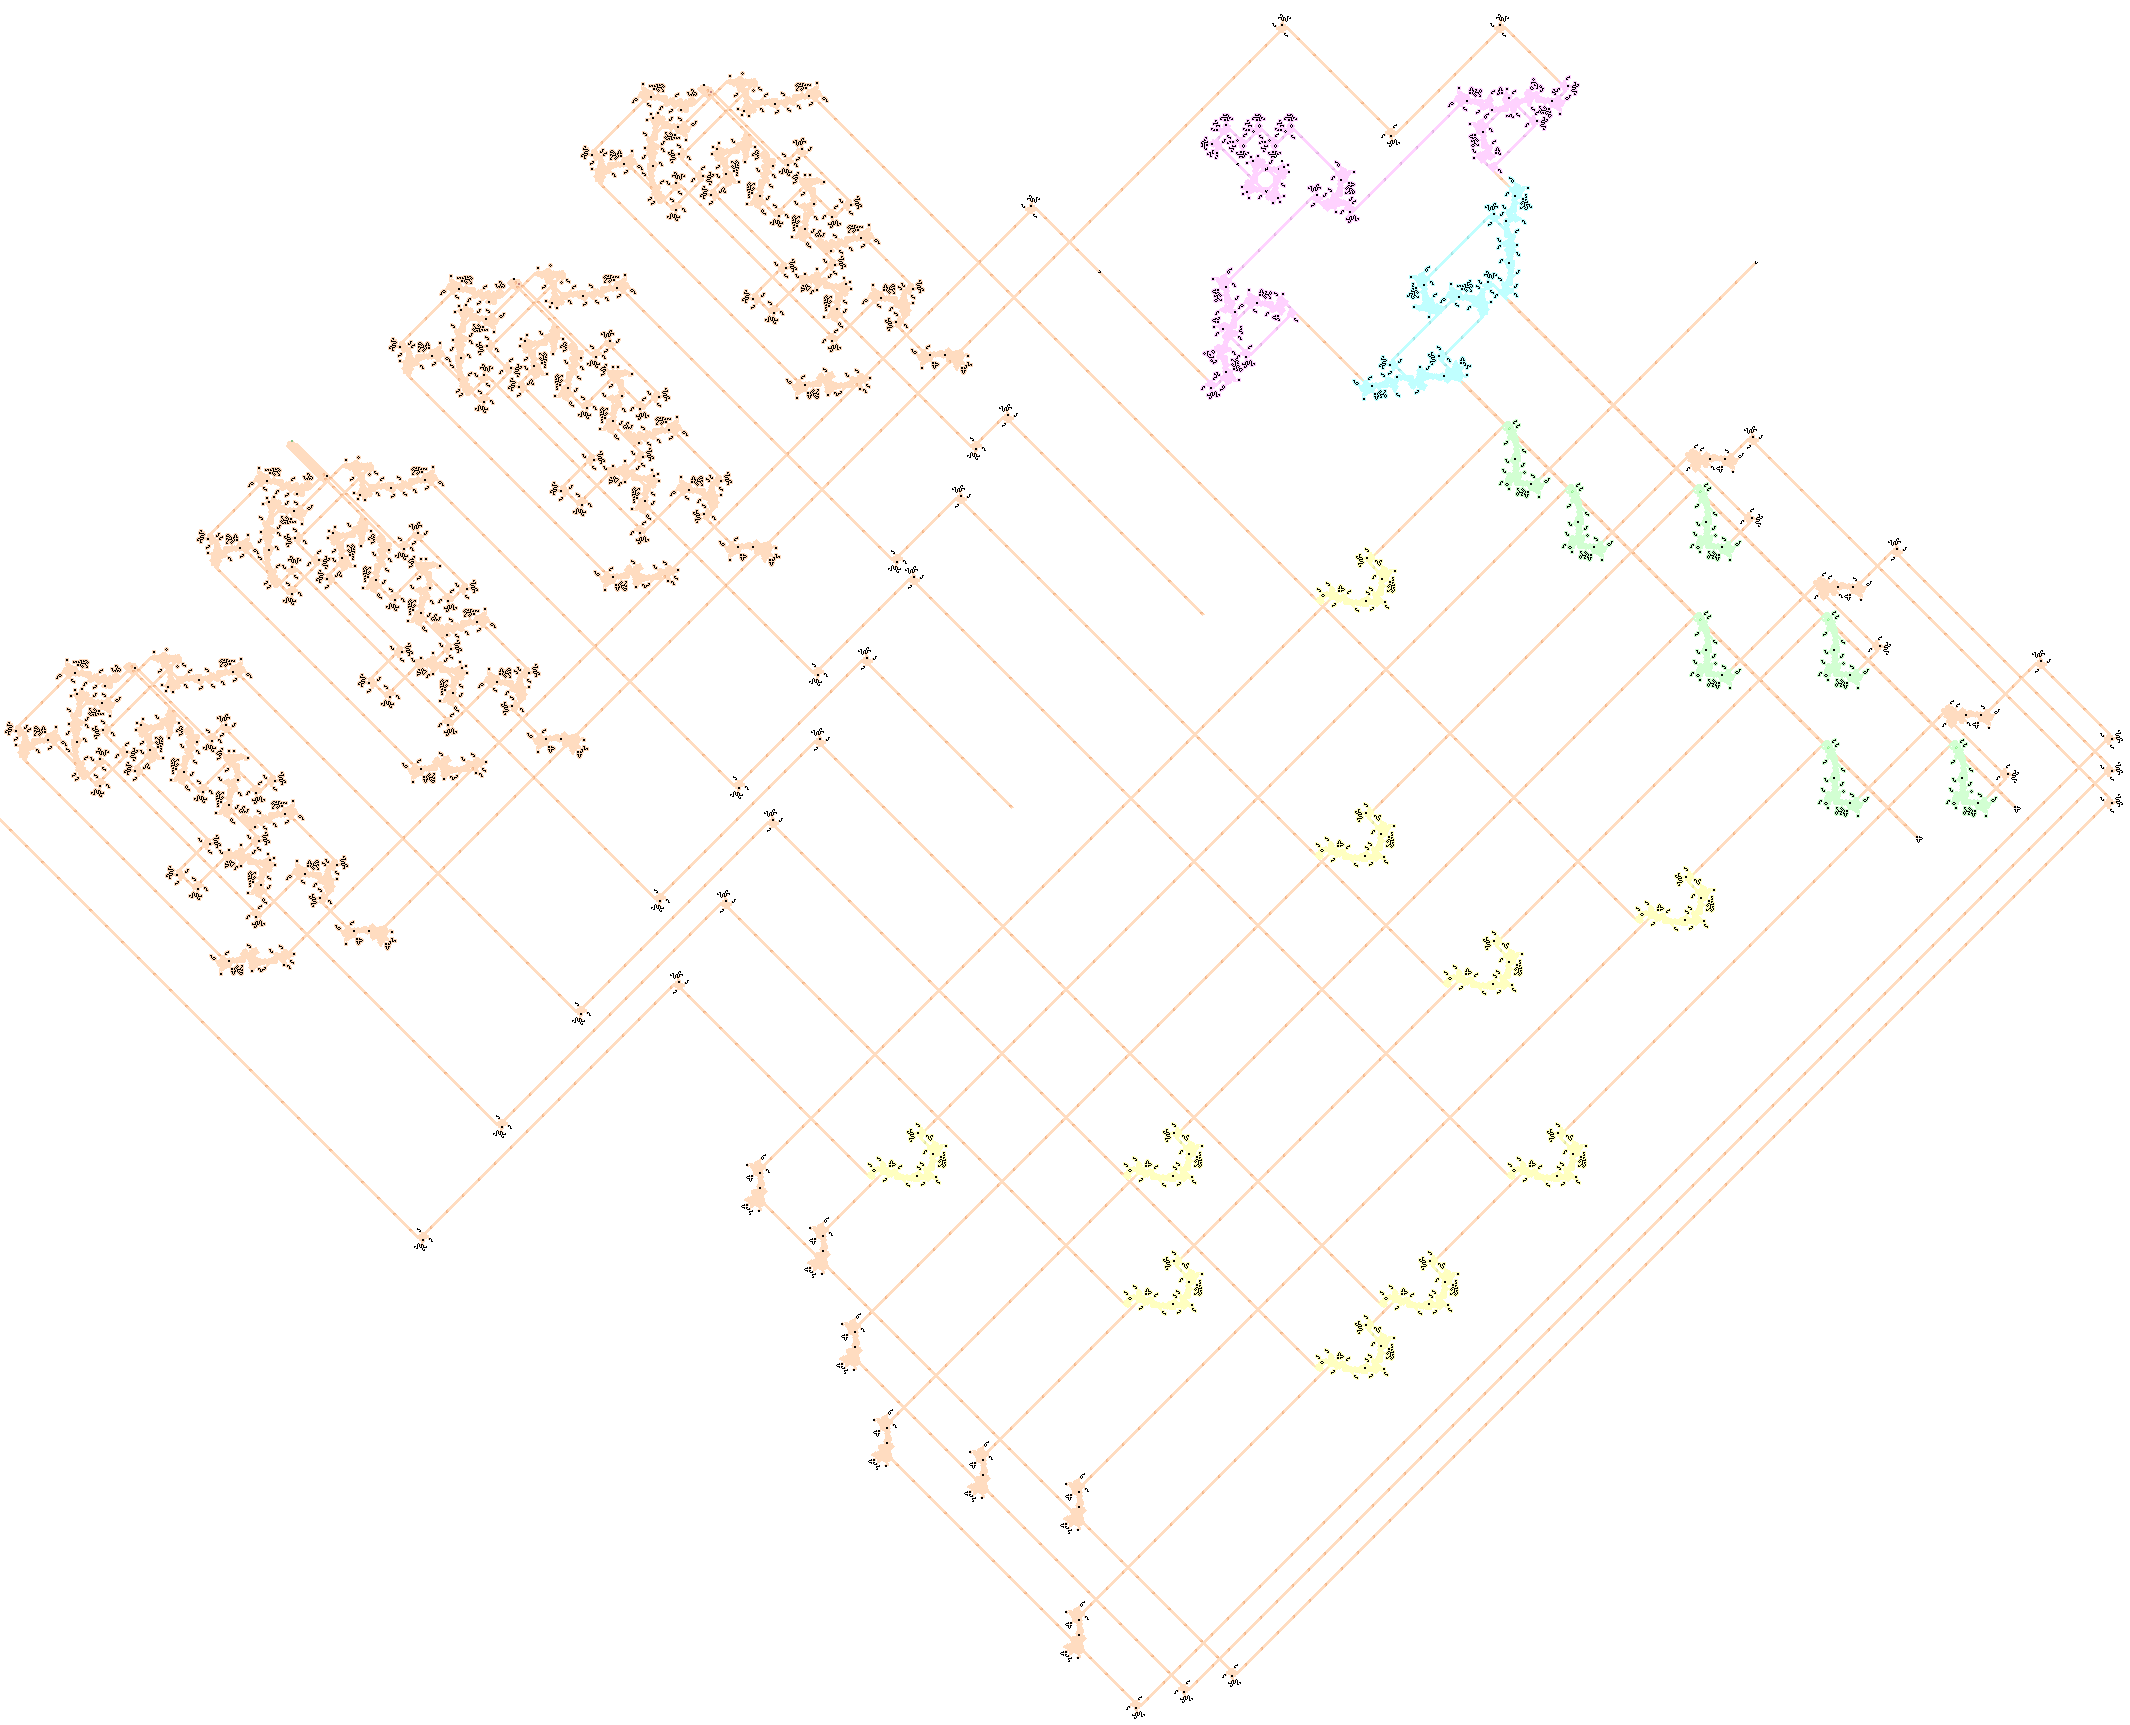
\includegraphics[width=12cm]{../universal_computation/mult_computer.png}};
		
		% Z OUT
		\newcommand\zoutx{5.63}
		\newcommand\zouty{8.62}
		\draw[gray] (\zoutx,\zouty) node[rotate=45] {\tiny \texttt{Z out}};
		\draw[color=gray,-stealth] (\zoutx-0.15,\zouty-0.3) -- (\zoutx+0.35,\zouty+0.2);
		
		% NZ OUT
		\newcommand\nzoutx{6.66}
		\newcommand\nzouty{9.24}
		\draw[gray] (\nzoutx,\nzouty) node[rotate=45] {\tiny \texttt{NZ out}};
		\draw[color=gray,-stealth] (\nzoutx-0.27,\nzouty-0.4) -- (\nzoutx+0.43,\nzouty+0.3);
		
		% Z IN
		\newcommand\nzinx{8.63}
		\newcommand\nziny{7.5}
		\draw[gray] (\nzinx,\nziny) node[rotate=-45] {\tiny \texttt{Z}};
		\draw[color=gray,-stealth] (\nzinx-0.18,\nziny+0.04) -- (\nzinx+0.09,\nziny-0.23);
		
		% NZ IN
		\newcommand\zinx{9}
		\newcommand\ziny{7.83}
		\draw[gray] (\zinx,\ziny) node[rotate=-45] {\tiny \texttt{NZ}};
		\draw[color=gray,-stealth] (\zinx-0.2,\ziny+0.06) -- (\zinx+0.13,\ziny-0.27);
		
		% HALT_OUT
		\newcommand\haltx{4.24}
		\newcommand\halty{3.77}
		\draw[gray] (\haltx-0.15,\halty-0.15) node[rotate=-45] {\tiny \texttt{HALT\_OUT}};
		\draw[color=gray,stealth-] (\haltx-0.45,\halty+0.31) -- (\haltx+0.24,\halty-0.38);
		
		% INC R3
		\newcommand\incrtx{4.56}
		\newcommand\incrty{4.17}
		\draw[gray] (\incrtx-0.15,\incrty-0.15) node[rotate=-45] {\tiny \texttt{INC R3}};
		\draw[color=gray,stealth-] (\incrtx-0.45,\incrty+0.31) -- (\incrtx+0.24,\incrty-0.38);
		
		% TDEC R3
		\newcommand\tdecrtx{4.88}
		\newcommand\tdecrty{4.57}
		\draw[gray] (\tdecrtx-0.15,\tdecrty-0.15) node[rotate=-45] {\tiny \texttt{TDEC R3}};
		\draw[color=gray,stealth-] (\tdecrtx-0.45,\tdecrty+0.31) -- (\tdecrtx+0.24,\tdecrty-0.38);
		
		% INC R2
		\newcommand\incrtwx{5.2}
		\newcommand\incrtwy{4.97}
		\draw[gray] (\incrtwx-0.15,\incrtwy-0.15) node[rotate=-45] {\tiny \texttt{INC R2}};
		\draw[color=gray,stealth-] (\incrtwx-0.45,\incrtwy+0.31) -- (\incrtwx+0.24,\incrtwy-0.38);
		
		% TDEC R2
		\newcommand\tdecrtwx{5.52}
		\newcommand\tdecrtwy{5.37}
		\draw[gray] (\tdecrtwx-0.15,\tdecrtwy-0.15) node[rotate=-45] {\tiny \texttt{TDEC R2}};
		\draw[color=gray,stealth-] (\tdecrtwx-0.45,\tdecrtwy+0.31) -- (\tdecrtwx+0.24,\tdecrtwy-0.38);
		
		% INC R1
		\newcommand\incrox{5.84}
		\newcommand\incroy{5.77}
		\draw[gray] (\incrox-0.15,\incroy-0.15) node[rotate=-45] {\tiny \texttt{INC R1}};
		\draw[color=gray,stealth-] (\incrox-0.45,\incroy+0.31) -- (\incrox+0.24,\incroy-0.38);
		
		% TDEC R1
		\newcommand\tdecrox{6.16}
		\newcommand\tdecroy{6.17}
		\draw[gray] (\tdecrox-0.15,\tdecroy-0.15) node[rotate=-45] {\tiny \texttt{TDEC R1}};
		\draw[color=gray,stealth-] (\tdecrox-0.45,\tdecroy+0.31) -- (\tdecrox+0.24,\tdecroy-0.38);
		
		% INC R0
		\newcommand\incrzx{6.48}
		\newcommand\incrzy{6.57}
		\draw[gray] (\incrzx-0.15,\incrzy-0.15) node[rotate=-45] {\tiny \texttt{INC R0}};
		\draw[color=gray,stealth-] (\incrzx-0.45,\incrzy+0.31) -- (\incrzx+0.24,\incrzy-0.38);
		
		% TDEC R0
		\newcommand\tdecrzx{6.8}
		\newcommand\tdecrzy{6.97}
		\draw[gray] (\tdecrzx-0.15,\tdecrzy-0.15) node[rotate=-45] {\tiny \texttt{TDEC R0}};
		\draw[color=gray,stealth-] (\tdecrzx-0.45,\tdecrzy+0.31) -- (\tdecrzx+0.24,\tdecrzy-0.38);
		
		% INITIAL; Z
		\newcommand\initzx{7.8}
		\newcommand\initzy{6.93}
		\draw[gray] (\initzx,\initzy) node[rotate=45] {\tiny \texttt{INITIAL;Z}};
		\draw[color=gray,stealth-] (\initzx-0.3,\initzy-0.45) -- (\initzx+0.42,\initzy+0.27);
		
		% ID1; Z
		\newcommand\idox{8.2}
		\newcommand\idoy{6.61}
		\draw[gray] (\idox,\idoy) node[rotate=45] {\tiny \texttt{ID1;Z}};
		\draw[color=gray,stealth-] (\idox-0.25,\idoy-0.4) -- (\idox+0.37,\idoy+0.22);
		
		% ID1; NZ
		\newcommand\idonx{8.56}
		\newcommand\idony{6.25}
		\draw[gray] (\idonx,\idony) node[rotate=45] {\tiny \texttt{ID1;NZ}};
		\draw[color=gray,stealth-] (\idonx-0.25,\idony-0.4) -- (\idonx+0.37,\idony+0.22);
		
		% ID2; Z
		\newcommand\idtwx{8.9}
		\newcommand\idtwy{5.87}
		\draw[gray] (\idtwx,\idtwy) node[rotate=45] {\tiny \texttt{ID2;Z}};
		\draw[color=gray,stealth-] (\idtwx-0.25,\idtwy-0.4) -- (\idtwx+0.37,\idtwy+0.22);
		
		% ID2; NZ
		\newcommand\idtwnx{9.26}
		\newcommand\idtwny{5.51}
		\draw[gray] (\idtwnx,\idtwny) node[rotate=45] {\tiny \texttt{ID2;NZ}};
		\draw[color=gray,stealth-] (\idtwnx-0.25,\idtwny-0.4) -- (\idtwnx+0.37,\idtwny+0.22);
		
		% ID3; Z
		\newcommand\idthx{9.77}
		\newcommand\idthy{5.3}
		\draw[gray] (\idthx,\idthy) node[rotate=45] {\tiny \texttt{ID3;Z}};
		\draw[color=gray,stealth-] (\idthx-0.25,\idthy-0.4) -- (\idthx+0.37,\idthy+0.22);
		
		% ID3; NZ
		\newcommand\idthnx{9.98}
		\newcommand\idthny{4.79}
		\draw[gray] (\idthnx,\idthny) node[rotate=45] {\tiny \texttt{ID3;NZ}};
		\draw[color=gray,stealth-] (\idthnx-0.25,\idthny-0.4) -- (\idthnx+0.37,\idthny+0.22);
		
		% CIRCLE THE INTIAL GLIDERS
		\draw[white,line width=1.5pt,opacity=0.6](6.51,8.38) circle (0.1);
		\draw[redback2,line width=0.6pt](6.51,8.38) circle (0.1);
		\draw[white,line width=1.5pt,opacity=0.6](9.902,8.243) circle (0.1);
		\draw[redback2,line width=0.6pt](9.902,8.243) circle (0.1);

		% COMPONENT STACK
		\draw[gridgray,dashed] (0,5.35) -- (0,5.8) -- (3.6,9.4) -- (4.75,9.4) -- (4.75,8.85) -- (5.8,7.8) -- (2.1,4.1) -- (1.25,4.1) -- cycle;
		\draw[gray] (3.3,5) node[rotate=45] {\scriptsize \texttt{Component Stack}};
		
		% COMPUTER
		\draw[gridgray,dashed] (8.8,7.4) -- (9.9,7.4) -- (10.5,6.8) -- (10.7,6.8) -- (11.3,6.2) -- (11.5,6.2) -- (12,5.7) -- (12,5.05) -- (6.95,0) -- (6.25,0) -- (4.65,1.6) -- (4.65,2.3) -- (4.1,2.85) -- (4.1,3.25) -- (4.2,3.35);
		\draw[gridgray,dashed] (5.55,4.6) -- (7.3,6.35);
		\draw[gray] (9.7,2.4) node[rotate=45] {\scriptsize \texttt{Computer}};
		
		% BORDER
		\draw[gridgray] (0,0) rectangle (12,9.72);
		
		% ZOOM BOX R0
			\newcommand\rzsmlx{3.93}
			\newcommand\rzsmrx{\rzsmlx+0.1945}
			\newcommand\rzsmby{9.13}
			\newcommand\rzsmty{\rzsmby+0.1945}
			
			\newcommand\rzbglx{3.6}
			\newcommand\rzbgrx{\rzbglx+1.552}
			\newcommand\rzbgty{11.05}
			\newcommand\rzbgby{\rzbgty-1.552}
			
			\path[draw,gridgray,line width=0.45pt] (\rzsmlx,\rzsmty) -- (\rzbglx,\rzbgty);
			\path[draw,gridgray,line width=0.45pt] (\rzsmrx,\rzsmty) -- (\rzbgrx,\rzbgty);
			
			\node[inner sep=0pt,anchor=north west] (zoom1) at (\rzbglx,\rzbgty) {
\includegraphics[width=1.552cm]{../universal_computation/mult_computer_zoom1.png}};
			
			\path[fill,white,opacity=0.4,line width=0pt] (\rzsmlx,\rzsmty) -- (\rzsmrx,\rzsmty) -- (\rzsmrx,\rzsmby) -- (\rzbgrx,\rzbgby) -- (\rzbglx,\rzbgby) -- (\rzsmlx,\rzsmby) -- cycle;
			
			\path[draw,gridgray,line width=0.45pt] (\rzsmlx,\rzsmby) -- (\rzbglx,\rzbgby);
			\path[draw,gridgray,line width=0.45pt] (\rzsmrx,\rzsmby) -- (\rzbgrx,\rzbgby);
			
			%\node[inner sep=0pt] (zoom1_3x) at (3.35,7.95) {
\includegraphics[width=0.21cm]{../mag.png} \footnotesize 8x};
			
			\filldraw[draw=gridgray,fill=white,line width=0.3pt,fill opacity=0.64] (\rzsmlx,\rzsmty) rectangle (\rzsmrx,\rzsmby);
			\draw[gridgray,line width=0.6pt] (\rzbglx,\rzbgty) rectangle (\rzbgrx,\rzbgby);
			
			\draw[gray] (\rzbglx,\rzbgty) node[anchor=north west] {\footnotesize \texttt{R0 = 7}};
			\draw[dred,opacity=0.5] (4.26,9.9) node[anchor=south west] {\footnotesize \texttt{0}};
			\draw[gray] (3.91,10.25) node[anchor=south west] {\footnotesize \texttt{7}};
		% END ZOOM BOX R0
		
		% ZOOM BOX R1
			\newcommand\ronesmlx{2.85}
			\newcommand\ronesmrx{\ronesmlx+0.1945}
			\newcommand\ronesmby{8.06}
			\newcommand\ronesmty{\ronesmby+0.1945}
			
			\newcommand\ronebglx{1.9}
			\newcommand\ronebgrx{\ronebglx+1.552}
			\newcommand\ronebgty{10.55}
			\newcommand\ronebgby{\ronebgty-1.552}
			
			\path[draw,gridgray,line width=0.45pt] (\ronesmlx,\ronesmty) -- (\ronebglx,\ronebgty);
			\path[draw,gridgray,line width=0.45pt] (\ronesmrx,\ronesmty) -- (\ronebgrx,\ronebgty);
			
			\node[inner sep=0pt,anchor=north west] (zoom1) at (\ronebglx,\ronebgty) {
\includegraphics[width=1.552cm]{../universal_computation/mult_computer_zoom2.png}};
			
			\path[fill,white,opacity=0.4,line width=0pt] (\ronesmlx,\ronesmty) -- (\ronesmrx,\ronesmty) -- (\ronesmrx,\ronesmby) -- (\ronebgrx,\ronebgby) -- (\ronebglx,\ronebgby) -- (\ronesmlx,\ronesmby) -- cycle;
			
			\path[draw,gridgray,line width=0.45pt] (\ronesmlx,\ronesmby) -- (\ronebglx,\ronebgby);
			\path[draw,gridgray,line width=0.45pt] (\ronesmrx,\ronesmby) -- (\ronebgrx,\ronebgby);
			
			%\node[inner sep=0pt] (zoom1_3x) at (3.35,7.95) {
\includegraphics[width=0.21cm]{../mag.png} \footnotesize 8x};
			
			\filldraw[draw=gridgray,fill=white,line width=0.3pt,fill opacity=0.64] (\ronesmlx,\ronesmty) rectangle (\ronesmrx,\ronesmby);
			\draw[gridgray,line width=0.6pt] (\ronebglx,\ronebgty) rectangle (\ronebgrx,\ronebgby);
			
			\draw[gray] (\ronebglx,\ronebgty) node[anchor=north west] {\footnotesize \texttt{R1 = 5}};
			\draw[dred,opacity=0.5] (2.57,9.39) node[anchor=south west] {\footnotesize \texttt{0}};
			\draw[gray] (2.32,9.66) node[anchor=south west] {\footnotesize \texttt{5}};
		% END ZOOM BOX R1
		
		% ZOOM BOX R2
			\newcommand\rtwosmlx{1.59}
			\newcommand\rtwosmrx{\rtwosmlx+2*0.193}
			\newcommand\rtwosmby{7.01}
			\newcommand\rtwosmty{\rtwosmby+2*0.193}
			
			\newcommand\rtwobglx{0.2}
			\newcommand\rtwobgrx{\rtwobglx+1.552}
			\newcommand\rtwobgty{10.05}
			\newcommand\rtwobgby{\rtwobgty-1.552}
			
			\path[draw,gridgray,line width=0.45pt] (\rtwosmlx,\rtwosmty) -- (\rtwobglx,\rtwobgty);
			\path[draw,gridgray,line width=0.45pt] (\rtwosmrx,\rtwosmty) -- (\rtwobgrx,\rtwobgty);
			
			\node[inner sep=0pt,anchor=north west] (zoom1) at (\rtwobglx,\rtwobgty) {
\includegraphics[width=1.552cm]{../universal_computation/mult_computer_zoom3.png}};
			
			\path[fill,white,opacity=0.4,line width=0pt] (\rtwosmlx,\rtwosmty) -- (\rtwosmrx,\rtwosmty) -- (\rtwosmrx,\rtwosmby) -- (\rtwobgrx,\rtwobgby) -- (\rtwobglx,\rtwobgby) -- (\rtwosmlx,\rtwosmby) -- cycle;
			
			\path[draw,gridgray,line width=0.45pt] (\rtwosmlx,\rtwosmby) -- (\rtwobglx,\rtwobgby);
			
			%\node[inner sep=0pt] (zoom1_3x) at (3.35,7.95) {
\includegraphics[width=0.21cm]{../mag.png} \footnotesize 8x};
			
			\filldraw[draw=gridgray,fill=white,line width=0.3pt,fill opacity=0.64] (\rtwosmlx,\rtwosmty) rectangle (\rtwosmrx,\rtwosmby);
			\draw[gridgray,line width=0.6pt] (\rtwobglx,\rtwobgty) rectangle (\rtwobgrx,\rtwobgby);
			
			\path[draw,gridgray,line width=0.45pt] (\rtwosmrx,\rtwosmby) -- (\rtwobgrx,\rtwobgby);
			
			\draw[gray] (\rtwobglx,\rtwobgty) node[anchor=north west] {\footnotesize \texttt{R2}};
			\draw[gren,opacity=0.5] (0.35,9.35) node[anchor=south west] {\footnotesize \texttt{35}};
			\draw[gray] (1.2,8.57) node[anchor=south west] {\footnotesize \texttt{0}};
		% END ZOOM BOX R2
		
		\draw[gray] (0.5,6.42) node[anchor=north west] {\footnotesize \texttt{R3}};
	\end{tikzpicture}
\end{document}